\chapter{Implementacja}
Przeanalizowanie problemu postawionego w niniejszej pracy magisterskiej wymagało implementacji własnych narzędzi. Jak wcześniej
wspomniano, programy dostępne w sieci są bardzo dobre (dig \cite{dig}, axfr-tool \cite{python_axfr_test}, robotex \cite{robotex})
jednak nie zapewniają oczekiwanej wydajności. Wynika to z faktu, że są one nastawione głównie na analizę konkretnego przypadku.
Narzędzia są używane głównie przez pentesterów, których typowym zadaniem jest przetestowanie pod kątem bezpieczeństwa na przykład pewnej
aplikacji, gdzie liczba serwerów DNS jak i testowanych domen jest mocno ograniczona. Proces ten sam w sobie jest niezwykle złożony
i często wymaga nawet tygodni pracy, dlatego czas w jakim wykonywał się będzie program sprawdzający podatności DNS nie jest aż tak
istotny. Oczywiście mówimy o różnicy w czasie w granicach do kilku minut. W podejściu prezentowanym w tej pracy założono, że
przeanalizuje się możliwie jak najwięcej domen dostępnych w sieci internet. Dlatego też różnica procesowania jednej pary
domena -- adres IP serwera autorytatywnego już nawet na poziomie kilku sekund pozwala zaobserwować bardzo duży skok wydajności.

Dojście do rozwiązania optymalnego nie było trywialne. Początkowe rozwiązania opierały się na próbach rozszerzenia dostępnych
narzędzi o managera
zarządzającego procesami, w których uruchamiane były zewnętrzne narzędzia -- głównie dig. Rozwiązanie takie miało szereg zalet,
na przykład było bardzo skalowalne i łatwe do zrealizowania. Niestety okazało się, że menedżer zarządzający procesami wymaga
zbyt dużej ilości zasobów, a głównie pamięci RAM, dlatego wymuszone zostało zrezygnowanie z tego podejścia.

\section{Przegląd dostępnych narzędzi}
Społeczność internetu oferuje bardzo szeroką gamę narzędzi umożliwiających pozyskiwanie informacji na podstawie protokołu DNS.
Bardzo użytecznym i przydatnym narzędziem jest w tym przypadku program dig. Wspomniany program ma jednak znaczącą wadę -- jest
wydajny jedynie przy niewielkiej liczbie odpytywanych domen. Dodatkową niedogodnością jest, wbrew pozorom, fakt, że program
wchodzi w skład pakietu Open Source bind. Ten, jak każde oprogramowanie na wolnej licencji, cierpi na szereg niedogodności z
tym związanych. Najbardziej prozaicznym problemem jest fakt, że oprogramowanie jest tworzone przez wiele osób, więc bardzo
trudno zastosować jeden standard kodowania, gdyż każda z osób ma swój preferowany. Poza tym, dużą wadą jest trudność wprowadzania
zmian w tego typu oprogramowaniu, wynikająca zarówno z punktu poprzedniego jak i ze złożoności programu, którą cechuje się dig
w tym momencie.

Istnieją także inne pakiety implementujące w dość wydajny sposób klienta systemu DNS jak np. pjlib \cite{pjlib}. Również w tym
przypadku można borykać się z problemami wynikającymi z założeń przyjętych przez twórców tego oprogramowania. Konkretyzując to
stwierdzenie - wspomniana biblioteka z założenia miała być wykorzystywana do protokołu SIP, a więc implementacja klienta DNS
weszła w jej skład tylko i wyłączenie dlatego, że twórcy jej potrzebowali jako narzędzia do zrealizowania innych celów.
Implikuje to fakt, że pobieranie wiadomości jest niekompletne na płaszczyźnie typów wiadomości. Jednym z nich jest typ nr 252,
czyli AXFR, który jest jednym z kluczowych elementów rekonesansu na podstawie protokołu DNS.

\section{Zaimplementowane narzędzia}
Przeprowadzenie globalnego skanu niosło za sobą szereg konsekwencji. Zakładając, że średnio należy przeznaczyć na skanowanie
jednej pary (domena, adres IP) około 3 sekund okazało się, że przeprocesowanie całego zbioru danych wejściowych (ok. 5 miliardów
par) zajęłoby odpowiednio:
$$3(s) * 5 * 10^{9} = 25 * 10^{8}(min) = \frac{25}{60} * 10^{8}(h) = 41.67 * 10^{6} (dni)\label{obliczenia}$$
Opierając się na opisanym wyżej rozumowaniu, podjęto decyzję, że należy procesować pary (domena, adres IP) równolegle.
Podjętych zostało kilka prób implementacji odpowiedniego narzędzia umożliwiającego przeprowadzenie badań w zadowalającym czasie:
\begin{itemize}
	\item narzędzie oparte na programie dig skryptach powłoki bash,
	\item menadżer procesów programu dig oparty na skryptach języka Python,
	\item skaner AXFR (C-AXFR) wspomagany skryptami powłoki bash.
\end{itemize}
Szczegółowo zostaną one opisane w kolejnych punktach tego rozdziału.

\subsection{Program dig zarządzany skryptami powłoki}
\label{dig_sh}
Pierwszym rozwiązaniem, które powstało w ramach pracy nad opisywanym problemem był skaner AXFR oparty na programie
dig \cite{isc}. Program skupia się wokół protokołu DNS i umożliwia wykonywanie zapytań różnych typów \cite{Liu:2006:DB:1197828}.
Ponadto, jest prosty w obsłudze, daje duże możliwości jeśli chodzi o budowanie zapytań DNS oraz bardzo często dostępny jest
domyślnie w wielu dystrybucjach systemów operacyjnych Linux.

Odpowiedzi uzyskane dzięki programowi miały być zapisywane do plików tekstowych. Każda, potencjalnie uzyskana odpowiedź miała
być zapisywana do oddzielnego pliku tekstowego, aby wykluczyć równoczesne użycie tego samego zasobu przez wiele procesów.
Rozwiązanie tego typu działa oraz z powodzeniem przeskanowano kilka tysięcy domen, jednak okazało się zbyt wolne do zastosowania
na szerszą skalę a także występowały kłopoty z zapotrzebowaniem na zasoby (mowa tu głównie o pamięci operacyjnej). Bliźniacze
podejście zostało zastosowane w opisywanym wcześniej projekcie skanowania domen z listy \textit{Alexa 1 Milion} \cite{scans.io}.

\subsection{Menedżer procesów zarządzany skryptami języka Python}
Kolejną próbą rozwiązania problemu ogromnej liczby danych do przeskanowania była implementacja skanera w języku skryptowym Python.
Próba ta podyktowana była kilkoma istotnymi aspektami. Pierwszym z nich jest implementacja tak zwanych ,,programowych'' wątków w
standardowej bibliotece tego języka. Umożliwiło to implementację mechanizmu, który pozwolił sprawdzić, czy maszyna dysponuje
takimi zasobami, które pozwolą na uruchomienie kolejnego wątku skanującego. Dodatkowym atutem jest tu także możliwość wywoływania
poleceń powłoki systemu Linux ze skryptu języka Python, a więc możliwe było wykorzystanie istniejącej już implementacji programu
dig \cite{isc}.

Niestety podobnie jak we wcześniej opisywanym przypadku, problemem okazały się ograniczenia czasowe spowodowane niewystarczającą
ilością zasobów. Program został przetestowany podczas kilkudniowego skanowania i zdołano odpowiednio:
\begin{itemize}
	\item przeanalizować kilka milionów par (domena, adres IP),
	\item pozyskać dane do wstępnej analizy podatności w skali globalnej,
	\item dwukrotnie zawiesić maszynę, na której wykonywano badania.
\end{itemize}

Pomimo, że implementacja w języku Python nie okazała się na tyle wydajna aby wykorzystać ją w badaniach przeprowadzonych w
ramach tej pracy magisterskiej, jest to dobrze narzędzie dla pasjonatów bezpieczeństwa sieciowego, którzy chcą skanować wiele
serwerów. Podejście takie zaprezentowane jest w kilku projektach, które można znaleźć w serwisie github na przykład
Python-AXFR-test \cite{python_axfr_test} lub skanowanie domen z Alexy wraz ze wstępną analizą wyników \cite{asg-axfr}. Liczba osób,
które śledzą wymienione wyżej projekty znajduje się w przedziale kilkudziesięciu osób. (?? Sporne) Również na tej podstawie możemy zakładać,
że temat bezpieczeństwa transferów strefy cieszy się zainteresowaniem wśród pasjonatów bezpieczeństwa sieci. (??)

Można przypuszczać, że oba projekty zrealizowane w języku Python \cite{python_axfr_test, asg-axfr} oferują podobną wydajność do
rozwiązania zaimplementowanego podczas realizacji pracy magisterskiej, jednak nie były prowadzone pomiary pod tym kątem. Brak
bezpośredniego porównania wynika z faktu, że prace Stephena Haywooda \cite{asg-axfr} były prowadzone niemal równolegle z realizacją
niniejszej pracy magisterskiej, zaś skrypt Python-AXFR-test \cite{python_axfr_test} jest jednowątkowy i nastawiony głównie na test
pojedynczych serwerów, więc jego wykorzystanie wymagałoby implementacji bardzo podobnego mechanizmu, który opisywany był na
początku tego rozdziału.

\subsection{Skaner C-AXFR}
Ostatecznie zdecydowano się na napisanie własnego narzędzia umożliwiającego transfer strefy DNS. Wybór padł na język
programowania C \cite{Kernighan:1988:CPL:576122} w wersji standardu C11 \cite{ISO9899}. Oczywiście aplikacje pisane w języku
C nie należą do rozwiązań prostych, jednak są bardzo dobrym kompromisem pomiędzy wysokim poziomem abstrakcji modeli programistycznych
i łatwością dostępu do interfejsów sieciowych. Ponadto język C charakteryzuje się dość dobrą szybkością działania, ze względu na
kompilację kodów źródłowych do kodu binarnego. Kryterium szybkości działania było jednym z kluczowych przy implementacji, co
pokazały poprzednie próby implementacji.

Rolę danych wejściowych programu mogą pełnić odpowiednio:
\begin{enumerate}
	\item plik tekstowy w formacie \textit{adres\_domeny}|\textit{IP\_serwera\_autorytatywnego},
	\item para parametrów wejściowych podanych w odpowiedniej kolejności - \textit{adres\_domeny IP\_serwera\_autorytatywnego}.
\end{enumerate}
Zdecydowano się na takie rozróżnienie z prostego powodu. Najistotniejszą kwestią prezentowanego rozwiązania było
zachowanie podobieństwa do programu dig, który jest wykorzystywany przez wiele osób. Dodatkowo, dużo łatwiej można testować
logikę programu na małych
porcjach danych i opcja numer 2. została w pewnym sensie funkcją debugową. Jako wspomniane dane testowe najczęściej wykorzystywana
była domena \textit{zonetransfer.me} \cite{zonetransfer}, której autor specjalnie umożliwia transfer strefy, aby uzmysłowić innym
ludziom zagrożenie wynikające z niepowołanego korzystania.

Logika programu jest bardzo prosta. Początkowo budowana jest jednostka APDU protokołu DNS z odpowiednimi danymi, a w szczególności
z poprawnie ustawioną flagą \textit{qtype} odpowiedzialną za identyfikację rodzaju zapytania DNS. Co ważne, mechanizm AXFR wymaga
używania nietypowego dla DNS protokołu TCP.

Komunikacja z serwerami autorytatywnymi została oparta na blokujących gniazdach TCP. Dodatkowo, zaimplementowany został autorski
mechanizm pozwalający na wykorzystywanie własnych limitów czasu żądania przed wysłaniem pakietu TCP. Wymagało to przełączania
gniazda na nieblokujący tryb pracy. Następnie wykorzystano funkcję \textit{select()}, która zwraca informację o tym, czy możliwe jest
rozpoczęcie pisania/czytania danych z instancji gniazda TCP. Dokładny algorytm działania został przedstawiony na rysunku \ref{fig:socketAlg}.

\begin{figure}[ht]
	\centering
	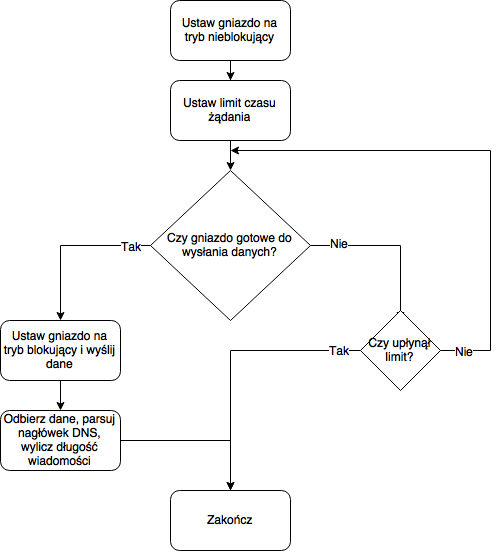
\includegraphics[width=1.0\textwidth]{image/socketAlg}
	\caption{Algorytm dynamicznego ustawiania limitu czasu żądania dla gniazda TCP w blokującym trybie pracy.}
	\label{fig:socketAlg}
\end{figure}

Program umożliwia parsowanie najbardziej popularnych i najczęściej używanych rekordów RR. Zostały one spisane w tabeli \ref{records}
wraz z identyfikatorami, które rezprezentują je w protokole DNS.

\begin{longtable}{|c|c|c|}
	\hline
	\textbf{Lp.} &
	\textbf{Typ rekordu} &
	\textbf{ID rekordu} \\ \hline\hline
	1 & A & 1 \\
	2 & AAAA & 28 \\
    3 & CNAME & 5 \\
	4 & HINFO & 13 \\
	5 & TXT & 16 \\
	6 & NS & 2 \\
	7 & SOA & 5 \\
	8 & PTR & 12 \\
	9 & MX & 15 \\
	10 & RP & 17 \\
	11 & AFSDB & 18 \\
	12 & LOC & 29 \\
	13 & SRV & 33 \\
	14 & NAPTR & 35 \\
	15 & RRSIG & 46 \\
	16 & NSEC & 47 \\
	17 & DNSKEY & 48 \\
	\hline
	\caption{Rekordy DNS obsługiwane w skanerze wraz z identyfikatorami.}
	\label{records}
\end{longtable}

Algorytm postępowania w przypadku odebrania pakietu danych przedstawiony jest na rysunku \ref{fig:receiving}. Dane odbierane z interfejsu
sieciowego są zapisane w systemie szesnastkowym, zgodnie z zaleceniami znanymi dokumentu RFC 1035 \cite{RFC1035}.

\begin{figure}[ht]
	\centering
	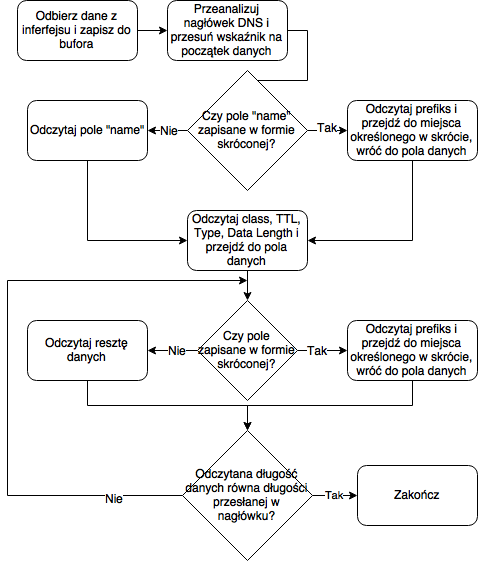
\includegraphics[width=1.0\textwidth]{image/receiving}
	\caption{Algorytm postępowania w przypadku odebrania APDU protokołu DNS.}
	\label{fig:receiving}
\end{figure}

Dodatkowo, jeśli zostanie odebrany typ, który nie został przewidziany w implementacji parsera to wszystkie dane odczytane z
socketa zostaną przeniesione w formie zapisu heksadecymalnego do pliku z odpowiedzią. Zapewnia ta kompatybilność z innymi
rozszerzeniami protokołu DNS oraz zabezpiecza przed błędnym wykluczeniem niektórych informacji ze skanowania. Jeśli pojawi
się nieznany wcześniej typ rekordu z bazy danych DNS, to będzie można interpretować go podczas analizy konkretnych odpowiedzi
od serwera.

Tak jak wcześniej wspomniano, transfer strefy DNS wykorzystuje protokół TCP, który nie jest tak powszechnie stosowany jeśli chodzi
o protokół Doman Name System. Wpływa to pośrednio na to, jakie wyniki możemy uzyskać przy próbie odpytania serwera o jego strefę. Mowa tu o
trzech charakterystycznych sytuacjach, mianowicie:
\begin{enumerate}
	\item brak możliwości nawiązania połączenia na warstwie 4 (TCP) na porcie 53,
	\item uzyskanie połączenia w rozumieniu protokołu TCP na porcie 53 i brak możliwości transferu danych,
	\item uzyskanie połączenia TCP na porcie 53 i pomyślny transfer danych.
\end{enumerate}

Początkowo założono, że uzyskanie już samego połączenia TCP z serwerem może być ciekawym przedmiotem badania. Interfejs serwera
autorytatywnego danej domeny powinien umożliwiać swoim klientom tylko kilka podstawowych operacji, jak na przykład translację nazwy
domenowej komputera ze swojej strefy na jego adres. Do takich działań połączenie TCP nie powinno być potrzebne. Dodatkowo, port 53 na którym działa
DNS jest zarezerwowany tylko dla tego protokołu, więc nie powinno udostępniać się na nim innych usług. Dowodzi to temu, że sytuacja,
gdy możliwe jest nawiązanie połączenia TCP na porcie 53 jest nienaturalna i niezgodna z panującymi dobrymi praktykami. Właśnie dlatego,
w pierwszej implementacji skanera założono, że program będzie tworzył puste pliki w przypadku opisanym w tym akapicie. Niestety,
zjawisko to okazało się tak powszechne, że powstały duże problemy związane z wydajnością skanera. Mowa tu o dostępie poszczególnych
procesów do dysku twardego maszyny na której były one uruchomione. Dlatego też zdecydowano się na zapisywanie informacji jedynie o
domenach, które odpowiedziały na zapytanie AXFR a sytuację umożliwiania nawiązywania sesji TCP na porcie 53 pozostawia się do analizy
podczas przyszłych badań.

Ostatecznie przyjęto rozwiązanie, które ignoruje fakt nawiązywania połączenia TCP oraz odpowiedzi od serwerów, w których nie ma
żadnych rekordów. Pozwoliło to na niemal dwukrotny wzrost wydajności zaimplementowanego skanera.

\section{Dane wejściowe}
\label{inputData}
Dane wejściowe programu zostały pozyskane od grupy naukowców z TU Delft \cite{delft} w formie par (domena, adres IP serwera
autorytarnego). Lista w takim formacie przechowywana była w pliku tekstowym. Zgromadzono w nim, zgodnie z tym co zostało przyjęte
w obliczeniach \ref{obliczenia}, ponad 5 miliardów wpisów uporządkowanych w kolejności alfabetycznej, a ich łączny rozmiar przekraczał
130 gigabajtów. Powoduje to oczywiście szereg problemów związanych z procesowaniem takich plików. (?? skad dane)

Jedną z niedogodności, które wiążą się z rozmiarem danych wejściowych był problem z wyborem losowej próby do kolejnych procesów
skanera. Pożądane jest, aby plik wejściowy do każdego z procesów skanujących nie był w żaden sposób uporządkowany, a najlepiej
gdyby dane w nim zawarte były wybrane losowo. Nie można założyć, że wszystkie procesy skanowania zakończą się bez żadnych błędów.
Jeśli więc dane wejściowe byłyby uporządkowane a proces zakończył się błędem wprowadzona zostanie dodatkowa, błędna korelacja między
brakiem odpowiedzi od serwera a nazwą domeny.

W systemach Linux dostępny jest domyślnie program \textit{shuf} \cite{shuf}, który dokonuje permutacji na konkretnych liniach w pliku,
jednak niemożliwe było wykorzystanie go wraz z plikiem z danymi wejściowymi z powodów ograniczeń wydajnościowych. Program nie był w
stanie zaalokować odpowiedniej liczby komórek w pamięci komputera. Aby zasymulować element losowości zastosowano algorytm zaprezentowany
na diagramie na rysunku \ref{fig:shufAlgorithm} oparty na dzieleniu całego zbioru danych wejściowych oraz permutowaniu kolejnych linii
w podgrupach o różnej wielkości.

\begin{figure}[ht]
	\centering
	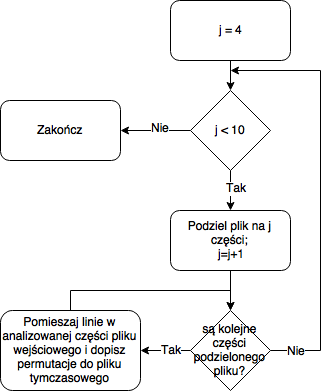
\includegraphics[width=0.6\textwidth]{image/sfuh}
	\caption{Algorytm mieszania linii w dużym pliku wejściowym.}
	\label{fig:shufAlgorithm}
\end{figure}

Następnie, plik został podzielony na mniejsze, po 25000 linii w każdym. Liczba linii w pojedynczym pliku została ustalona arbitralnie,
tak aby widoczny był postęp w skanowaniu. Przeprocesowanie 25 tysięcy linii odpowiada maksymalnie około 28 godzinom przy założeniu,
że dla każdej domeny upłynie limit czasu żądania.

\section{Środowisko uruchomieniowe}
Każda z aplikacji była rozwijana w podobny sposób. Cały proces można podzielić na 3 główne etapy:
\begin{enumerate}
	\item rozwijanie oprogramowania -- dodawanie nowych funkcji do skanera oraz proste testy funkcjonalne,
	\item uruchomienie w warunkach testowych -- sprawdzanie poprawności działania systemu w dłuższej perspektywie (do kilkunastu godzin),
	\item uruchomienie w środowisku docelowym -- właściwe skanowanie maksymalizujące wydajność.
\end{enumerate}
Ze względu na wygodę, każdy z etapów był uruchamiany na innej maszynie. Dostępność sprzętu była ograniczona, dlatego nie udało się
zapewnić, że każda z faz zostanie uruchomiona na takim samym urządzeniu. Faza pierwsza realizowana była na komputerze z procesorem
dwurdzeniowym Intel Core i3-4150, 8GB pamięci RAM oraz 1TB dyskiem twardym w zestawieniu ze 120GB dyskiem SSD. Etap uruchomienia systemu w
środowisku testowym przebiegał na maszynie z procesorem Intel Core2Duo E6420 z dwoma rdzeniami, 4GB pamięci RAM oraz 320GB dyskiem twardym. Etap ostatni,
właściwe skanowanie domen odbywało się na serwerze dedykowanym wypożyczonym od firmy OVH. Zaopatrzony był on w czterordzeniowy
procesor Intel Xeon E3-1230v6, 16GB pamięci RAM oraz 2x4TB dysk twardym.

Każda z maszyn działała pod kontrolą systemu operacyjnego opartego na dystrybucji systemu Debian. Podejście do problemu
w zaprezentowany sposób pozwoliło na szereg udogodnień. Pierwszy etap jest dość oczywisty -- nie ma sensu uruchamiać całego systemu
na serwerze, jeśli nie mamy pewności, że poszczególne komponenty w samym skanerze nie są odpowiednio zaimplementowane. Mylące może
być wprowadzenie etapu uruchomienia systemu w środowisku testowym. Powodem przyjęcia takiego rozwiązania były kwestie finansowe.
Nie mając pewności, że system działa dobrze w długiej perspektywie, nie warto było wypożyczać dedykowanego serwera jedynie do testowania.
W momencie, gdy można było domniemywać, że system działa stabilnie przez dłuższy okres, można było wypożyczyć serwer i skupić się
na uzyskaniu jak największej wydajności skanera.

\section{Metodyka badań}
Skaner został zaprojektowany w takie sposób, aby potrafił przeskanować kilka domen podczas jednego uruchomienia. Założenie wynika z
ograniczeń wydajnościowych, które zauważono przy próbie implementacji skanera, którą opisano w punkcie \ref{dig_sh}.

Skanera nie zaprojektowano tak, aby wspierał wielowątkowość. Może się okazać, że implementacja uruchamiania wielu wątków już w programie
będzie jeszcze bardziej wydajna niż proponowana w niniejszej pracy. Mimo to, opisywana propozycja zakłada realizację wielowątkowości
poprzez uruchomienie wielu procesów programu w systemie linux, każdy z inną listą domen do przeskanowania jako argumentem wejściowym.
Generacja poszczególnych list została opisana we wcześniejszym podpunkcie \ref{inputData}.

Pełen scenariusz skanowania zaprezentowano poniżej.
\begin{eumerate}
	\item Pobierz listę do skanowania.
	\item Wygeneruj N podzbiorów rozłącznych dla listy.
	\item Dla każdego podzbioru uruchom proces skanera z odpowiadającą mu listą.
\end{eumerate}

W prezentowanym przypadku liczba podzbiorów była bardzo duża, więc zdecydowano się na ograniczenie liczby uruchamianych procesów
skanera jednocześnie. Eksperymentalnie ustalono, że liczba instancji skanera na poziomie 15000 jest akceptowalna zarówno ze względu
na wydajność jak i stabilność. 

\section{System powiadomień}
W ramach badań przeprowadzonych podczas realizacji niniejszej pracy magisterskiej został zaimplementowany i uruchomiony system
powiadamiania administratorów domen. System bazuje na informacjach pobranych podczas skanowania podatności serwerów na zapytania
typu AXFR. W rekordzie SOA przesyłanym na początku i na końcu wiadomości przesyłany jest adres osoby odpowiedzialnej za daną domenę.
Jego miejscem jest pozycja numer 2. w rekordzie SOA z tą różnicą, że pierwszy znak ,,.'' napotkany w adresie jest zamieniany na
znak ,,@''. W wyniku tej zamiany uzyskiwany jest adres mailowy, przypisany do administratora domeny.

System powiadomień zaimplementowano w systemie operacyjnym z rodziny systemów UNIX. Opiera się on głównie na skryptach powłoki
\textit{bash}. Algorytm wyodrębnia rekordy SOA i wypisuje je do pliku. Następnie plik sortowany jest ze względu na adres mailowy
administratora domeny, po czym grupuje się te domeny, za które odpowiada ten sam adres pocztowy. Kolejnym krokiem jest pogrupowanie
domen oraz utworzenie odpowiedniego pliku tekstowego. Zawarte są w nim domeny oraz adresy serwerów które umożliwiają transfer
strefy dla danej domeny. Nazwa pliku odpowiada adresowi mailowemu zarządcy domeny.

Po otrzymaniu zbioru plików opisanych powyżej uruchamiany jest proces, którego zadaniem jest wysłanie wiadomości pod określone
adresy. Skrypt, który automatyzuje opisaną czynność napisano w języku Python \cite{python}. Wysyłane wiadomości podpisywane są
kluczem PGP \cite{RFC4880}, aby odbiorca mógł zweryfikować, że wiadomość została odebrana dokładnie w takiej formie jak ją przygotowano
i wysłano.
